% Chapter 3

\setcounter{chapter}{2}
\chapter{Spectral Trandformation}
\thispagestyle{plain}

%Box with Learning objectives should be at the beginning of each chapter
\begin{corollary}

	\hspace*{10mm}
	
	\vspace{5mm} %for optical corrections
	% optionaler Text	
	
	\begin{itemize}
		
			\item Fourier transformation (continuous time vs. discrete time)
			\item Digitization of speech signals (time-amplitude)
			\item Discrete Fourier Transform (DFT)
			
	\end{itemize}
\end{corollary}
\newpage

% CHAPTER 3 LESSON 1
\clearpage
\section{Fourier transformation (continuous time vs. discrete time)}
\label{Fourier transformation (continuous time vs. discrete time)}


%Einf�hrung in das Kapitel

Usually in signal processing, what we would like to do is modify a signal to some extent. For this it is important that the properties we want to modify are easily accessible. In the previous chapeter, we already saw that the fundamental period is an example of a speech property that is not so easily accesible in the time domain. It can be seen in the time domain, however it was shown that time domain based algorithms (ie.peak and zero crossing measurement) are prone to errors. It can then be beneficial to look at some transformation of the signal. Using the example of fundamental frequency estimation, it was shown that the autocorrelation function makes the estimation of the fundamental period more robust. A different concept is to look at the frequency content of signals. For instance, we have already seen some spectrograms of voiced speech. These produce a time/frequency based visualization that allows us to see the fluctuation of the spectral envelope.  It was shown that the spectral envelope is formed by the vocal tract and corresponds to the meaning of a sound and is what we use to distinguish between two phonemes. A narrow-band spectrogram can also reveal the fundamental frequency and its harmonics.  \\

This process of decomposing a signal into its frequency contents in order to make certain signal properties more accesible is known as Fourier theory. In Fourier analysis a signal is basically correlated with complex exponential functions, and because any exponential function can be written as a sum of cosine and sine functions, this means that it is correlated with cosine and sine functions. Because these exponentials can be shown to be linearly independent of each other(eigenfunctions), Fourier anaylsis preserves all of the original information and is therefore a completetly invertible function. This implies that no information is added or removed in the analysis and that it is simply a different way of representing the signal.  Certain attributes of the signal are made more visible whereas others are not visible any more. \\

 A pure tone is a tone that consists of only one sinusoid with a certain amplitude, frequency and phase. Note that this also includes a cosine function as a cosine is just a sine with a 90° phase shift. This pure tone is what we call a sinusoidal signal, and one of the key concepts of Fourier theory is that any periodic signal can always be represented as a sum of weighted sinusoids at the signals fundamental frequency and its harmonics, integer ultiples of the fundamental frequency. This is known as a Fourier series analysis.  Fourier theory can also be extended for arbitrary (non periodic) signals. The signal can then be shown to be composed of the integral over all frequencies that are in the signal, the spectrum of the signal.  This process is known as a Fourier analysis. \\

Figure 3.1 shows an example of a fourier series analysis of a rectangular function. The top sinusoid depicts the contribution of the fundamental period to the analysis. The second signal is the sum of the fundamental and a weighted third harmonic. It can be seen that the sum is a bit more close to the rectangular function, and as the number of harmonics is increased, a better approximation to original signal is achieved. The figure on the right shows how to weight the harmonics to get as close as possible to the square wave, and it can be seen that the majority of the energy is in the fundamental frequency with an exponential decay for the higher harmonics.  Another way of thinking about it is that at the edges of the rectangular function, there is a very sudden jump in the time domain, corresponding to a very high frequency content. Theoretically, one would need infinitely many harmonics to model the signal perfectly.\\

\begin{wrapfigure}{r}{0pt}
    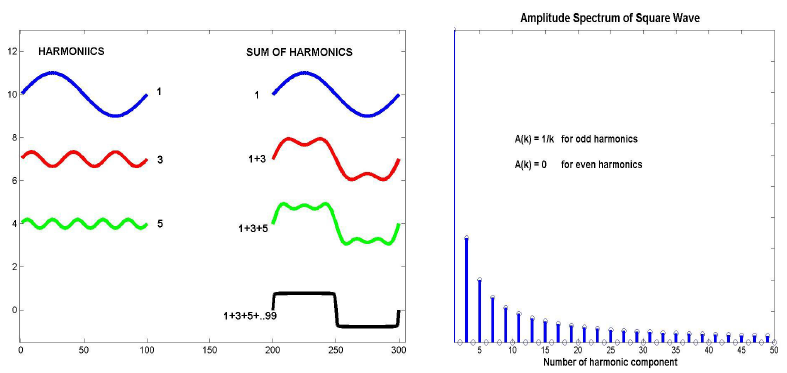
\includegraphics[width=0.7\textwidth]{Pictures/Chapter3_Lesson_1/FourierSquare.png}
    \caption{Fourier series analysis of a square wave.}
\end{wrapfigure}

Equation 3.1 is the mathematical representation of this process. The value, \begin{math}\cosCoef_0\end{math}, is called the DC offset and is the mean value about which the signal oscillates, in this case it is zero. The signal is therefore represented by this DC offset, and weigted contributions of sine and cosine functions at multiples of the fundamental frequency of the original signal. These weights are determined by correlating the original signal with cosine functions to determine the coefficients  \begin{math}\cosCoef_h\end{math} and sine functions to determine the coefficients \begin{math}\sinCoef_h\end{math}. Because the cosine function is an even function, whereas the rectangular function is odd, there will be zero correlation between the two. Therefore, the \begin{math}\cosCoef_h\end{math} coeffficients will all goto zero, leaving only the \begin{math}\sinCoef_h\end{math} coefficients to represent the signal. This can be seen in the right of Figure 1 along with the exponential decay of the weighting of the higher harmonics. \\

   \begin{tikzpicture}
\node [mybox] (box){%
    \begin{minipage}{0.50\textwidth}
    \begin{center}
    \begin{equation}x(t) = \frac{\cosCoef_0}{2}+\sum^{\infty}_{h=1}(\cosCoef_h\cos(2\pi hf_0t))+(\sinCoef_h\sin(2\pi 		hf_0t))
    \end{equation}
    \end{center}
  \end{minipage}
};
\node[fancytitle, right=10pt] at (box.north west) { Fourier series analysis};
\end{tikzpicture}%
  


Another reason why frequency analysis is a tool so often used in audio processing is that we also perceive sound in the frequency domain. This was introduced in the section on hearing regarding the frequency decomposition performed in the inner ear at different positions along the cochlea. This place coding implies that the cochlea performs a mechanical frequency analysis and that humans, in a sense, perceive sound in the frequency domain. This is the reason that it is quite natural for us to look at audio signals in the frequency domain. Computation can also be made much simpler in the spectral domain as convolution in the time domain corresponds to multiplcation in the frequency domain. This is often much easier to compute and is also another reason why spectral analysis can be the right tool to analyze certain signals.\\
  
  
  
%  
%  This is an example to get an idea of what frequency means what you can do is take a speech signal and filter out certain frequencioes andthen you get an idea of there certain contribuitions. SO this for instance is a speech signal with an audio bandwidth od 4khz. So if you throw away the frequencies higher than 2 khz we can stil understand but it doesnt sound nice anymore.  If we just look at the high frequency part, we only herar very little and it rather difficult to undertand and this is also because important formans are missing nowAnd if we just cut out frequencies between 500 and 1500Hz you can also get some odd distortions as opposed to the original.

  \begin{tikzpicture}
\node [mybox] (box){%
    \begin{minipage}{0.50\textwidth}
    \begin{center}
    \begin{equation*}
    X(\jmath\omega) = \int_{-\infty}^\infty x(t)e^{-\jmath \omega t} \mathrm{d}t
    \quad\quad\quad\quad x(t) = \frac{1}{2\pi} \int_{-\infty}^\infty X(\jmath \omega) e^{\jmath \omega t} \mathrm{d} \omega
    \end{equation*}
    \end{center}
  \end{minipage}
};
\node[fancytitle, right=10pt] at (box.north west) {Continuous-time Fourier transform};
\end{tikzpicture}%
   
    
  However, not all signals are periodic and eligible for Fourier series analysis.  In these cases, the continuous-time Fourier transform (Eq 3.2) can be used to represent any arbitrary signal. Any continuous time domain signal can be represented by a continuous frequency domain signal by bascially correlating the signal with complex exponentials over all frequencies, \begin{math}\omega\end{math}. And because complex exponentials can be represented with sines and cosines, this is like correlating the signal with sine and cosine functions over all frequencies, \begin{math}\omega\end{math}. In this sense, it is somewhat similar to the computation of the Fourier series coefficients, however the difference is that we now correlate over an infinite number of frequencies, not just the fundamental frequency and its harmonics.\\
  
   \begin{tikzpicture}
\node [mybox] (box){%
    \begin{minipage}{0.50\textwidth}
    \begin{center}
    \begin{equation*}
     X(e^{\jmath\omega}) = \sum_{\timei =-\infty}^\infty x(\timei ) e^{-\jmath \timei \omega}
      \quad\quad\quad\quad
      x(n) = \frac{1}{2\pi} \int_{-\pi}^\pi X(e^{\jmath\omega}) e^{\jmath\timei\omega}\mathrm{d} \omega
    \end{equation*}
    \end{center}
  \end{minipage}
};
\node[fancytitle, right=10pt] at (box.north west) {Discrete-time Fourier transform};
\end{tikzpicture}%
  
   
  
 The signals that we will be dealing with in digital speech processing will not be continuous, but discretized and sampled in the time domain.Therefore, we define the discrete time Fourier transform, DTFT. This is a transform with a discrete time index, \begin{math}\timei\end{math} but still a continuous frequency representation, \begin{math}\omega\end{math}. Here again,\begin{math}\omega\end{math} can take on an infinite number of values between 0 and \begin{math}2\pi\end{math}, wheras \begin{math}x(\timei)\end{math} is a finite,discrete representation of the original continuous signal. \\
  
    There are certain properties of the DTFT that can be related to the continuous time Fourier transform.  Looking at the definition of the DTFT in Eq2, we begin with the discrete time domain signal, \begin{math}x(\timei)\end{math}. To compute the frequency representation, instead of an integral, there is a summation.  The discrete time domain signal, \begin{math}x(\timei)\end{math} is  multiplied by phase shifted complex exponential functions and then summed. It is also important to note that, for the DTFT,  \begin{math}\timei\end{math} can only take on integer values. To return to the time domain, you would integrate over all frequencies again multiplied with these complex exponentials (conjugate?). Again these two transforrms are perfectly invertible meaning that there is no information lost upon conversion from time to frequency domain and vice versa.\\
    
 Because an integral and a summation are linear operators, the Fourier transform is itself linear. If you have a signal corresponding to the linear superpostion of two other signals, possibly even weighted with some scalar, then the Fourier transform of the sum of the two signals is equivalent to the sum of the Fourier transform of each signal. This is the basic defintiion of linearity and how we define a linear system. \\
  
 Very often in digital speech processing, we look at real valued signals in the time domain.  For example, a recording of an audio signal is real valued, implying that the spectrum is complex conjugate symmetric. This means that the real part is even while the imaginary part is odd. We can therefore also look at the even and the odd parts of the time domain signal separately. As introduced before, if  an even signal is correlated with a complex exponential, it is correalted with an even function, a cosine, and an odd function, a sine. The correlation between an even function and an odd will goto zero because of their opposing symmetries. When multiplied by the sine function, all values to the right of the origin will have equal, but opposing values, to the left of the origin, and the sum of the two will goto zero. \\
 
% So this means that the odd part of signal corresponds to the imaginary part of a spectrum.
% 
% Then a very basic property ist that the convolution, this is something you should all know.  A convolution in the time domain corresponds to a multiplecation in the frequency domain.
 
% Then a time shift, if you shift your signal in time, it corresponds to a taking the spectrum of a signal and modulating it with a omeag times the time shift.   It also goes the other way around if you shift your signal in the frequenccy domain, you have to modulate you signal in time domain. All of this properties are quite simple to derive.  All you have to do is the definitions of the FOurier transform and plug them in on one of the sides, and then you can derive all of these relations quite easy.  The last one is Parsevals theorem which also says the energy in a signal will be preserved when you take the Fourier analysis of a signal.


    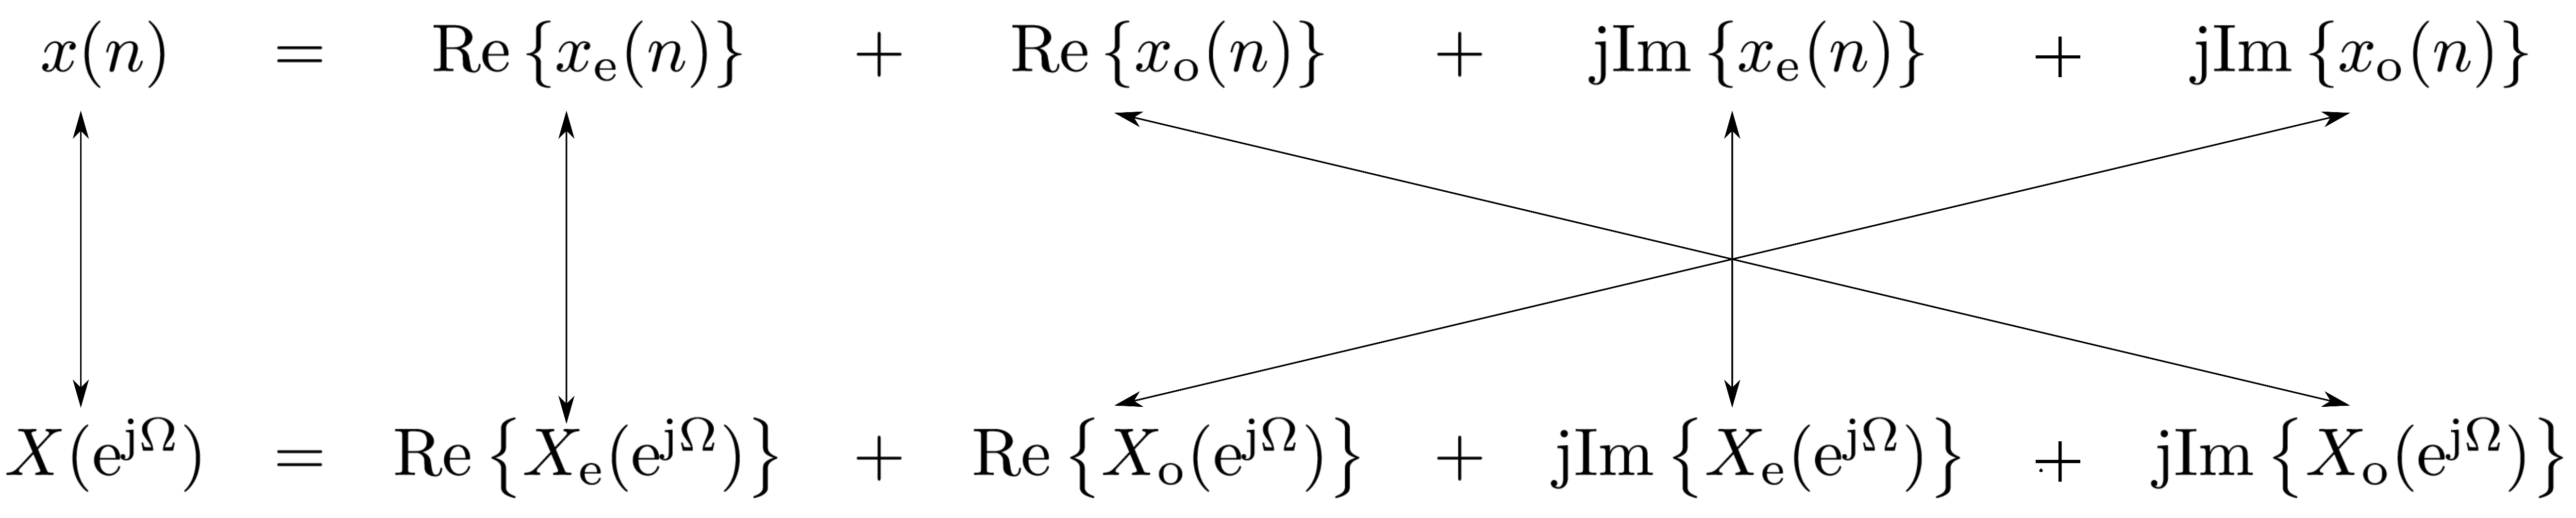
\includegraphics[width=0.7\textwidth]{Pictures/Chapter3_Lesson_1/dftSymmetry2-eps-converted-to.pdf}
   
 
 So, symmetry relations.  So this again relates to the analysis of the even and the odd part that I talked about before.  SO of coure, you can take a signal and it Fourier transform and you get the complex valued signal in the spectral domain . As we said, if you have areal valued and even signal, this corresponds to a real valued and even signal in the spectral domain.  However if real valued and odd signal, this corresponds to an imaginary and odd signal in the spectral domain. This is the representation that we will be working with most. Mostly we will be working with real valued signals meaning that you have a complex conjugate symmetric spectrum.  You could also make the same relations for complex signals then you would see that the the even paret of the imaginary part of a signal correposnds to the imaginary part of the spectrum, while the imaguinary parrtr and odd part corresponds to the reall value, but odd part of the specrtum.
 
 There are more relations in the spectral domain, and that is that whenever you have a discret time signal, this corresponds to a periodic spectrum and vice versa, if you have periodic signal, you would get a discrete spectrum. And when you kow this, you can do all  combinations of the two properties, for instance, if you have  continuous time signal that is not periodic. Also in the spectral domain, you would have a continuous spectrum that is not periodic. Then, if you have a continuos time signal that is periodic, for instance a vowel, you would have a discreter frequency and non periodic spectrum.  SO why when I have a vowel and lets say I do y frequency analysis why would I have a discrete frequency spectrum, or how would these discrete frequencies look.  The answer is that there are periodicites in the time domain signal corresponding to the fundamental period and its harmonics.  A frequency analysis of thi swould reveal discretized peaks in the spectral domain. So also if you have a discrete time signal, but also periodic at the same time, you would also have a discrete and periodic signal in the spectral domain and if you had a discrete signal that is not periodic, you would have a continous frequency spectrum, but periodic. So all of these four relations just stem from the two above. Here is a visualtization:
 
This is also important ot know, that if you have arectangular function, that in the fourier domain it corresponds to a synch function in the spectral domain.



% CHAPTER 3 LESSON 2
\clearpage
\section{Digitization of speech signals (time-amplitude)}
\label{Digitization of speech signals (time-amplitude)}

Spectral transformation, digitation of speech and audio signla.s This is what we are really aiming for. So what we would have is a microphone somewher in the room and now we speak into the microphone and eventually what you would do if you would like ti store the signal on a diital device or would like to transmit it through a digital channel  for instance a cell phone, we would firat need to digitalize the signal which involves a discretization of the time axis, so how is this done .

First of all if you have a signal and you would like to discretize it. It basically means that you take snaphots a certain unstances in time  and when you look at such a signal, it basically means that you dont really know what goes on inbetween two samples.  Then, the sampling theorem tellls you that if you have a sample rate that is high enough, you can still perfectly reconstruct you signal. Of copurse in sampling, you would like to use as few samples as possible because if you have too many sampling points, that would e a redundancy and that would be a waste of data storage, if you wanted to sotre the signal on a computer, or if you wanted to transmit the signal then the data rate that we would need would be too high. SO we want the sampling frequency to be as low as possible.And theit is important to understand how low you can go.

Sampling:

If you discretize a signal, you can think of it as the multiplecation of signal with a delta comb or an impulse train.  Now we want to understand what goes on in the frequency domain. We can use the property that the multiplecation in time domain corresponds to convolution in frequency domain. Because then,m if you know this you can compute the spectrum of the original signals, and loko at the result. And from this we can derive the necessary conditions that we need to fulfill in order to reconstruct our signal perfectly..

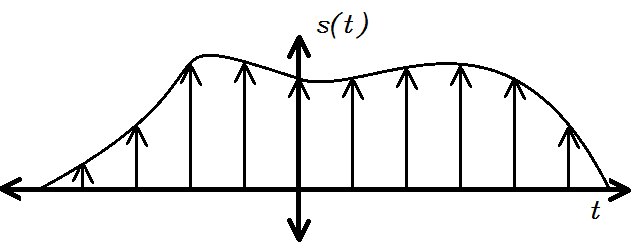
\includegraphics[width=0.5\linewidth]{Pictures/Chapter_2_Lesson_1/Sampling4.png}

So lets assume that we obtain our discrete signal by multiplying our signal with an impulse train:

\begin{equation*}\discFunc(\sampTime) = \contFunc(\sampTime)\cdot\Sh(\frac{\sampTime} {\samplingPeriod})\text{          with \begin{math}\samplingPeriod = \frac{1}{\samplingFreq}\end{math} the sampling period }\end{equation*}

The impulse train is given as a series of delta pulses spaced at Ts:

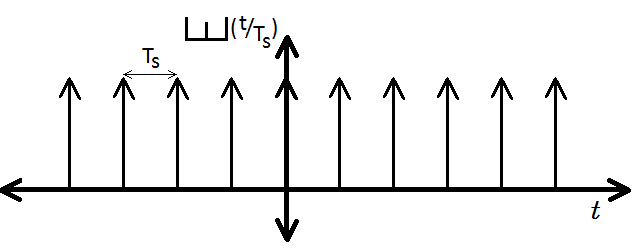
\includegraphics[width=0.5\linewidth]{Pictures/Chapter_2_Lesson_1/Sampling1.png}

So this signal is difined as the sum over infinitely many pulses(delta functions). And the are spaced at a distance of Ts and now here we have multiples of Ts and we have infinitley many that extend into positive and negative time domain.
 
 \begin{equation*}\Sh(\frac{\sampTime} {\samplingPeriod}) = \sum_{\sampIndex}\deltaPulse(\sampTime - \sampIndex\samplingPeriod) \end{equation*}
 
 And now we want to compute the spectrum of this signal.  So to do this we compute the integral over the signal multiplied with the complex exponentials which is basically the definition of the FOurire transform.
 
  \begin{equation*}\fourierSym( \Sh(\frac{\sampTime} {\samplingPeriod})) = \int^{\infty}_{-\infty}\sum_{\sampIndex}\deltaPulse(\sampTime - \sampIndex\samplingPeriod)e^{-jwt}dt  \end{equation*}
 
So how can we solve this integral? Well for instnce by using the sifting property.  This basically states taht if you take the integral of some function f(t) times a shifted impulse, and you integrate over all t, its corresponsd to evaluating the fuinction only at the point T.

\boxed{\int f(t)d(t-T)dt = f(t)\text{      ''Sifting Property''} }

But from because sums and integrals are linear terms, we can shift them.  And then what we get is the sum over infintiely many shifted complex exponential functions:

\begin{equation*}= \sum^{\infty}_{\sampIndex=-\infty} e^{-jw\sampIndex\samplingPeriod} \end{equation*}

So now we have this summation over exponential functions over infinitely many n. So what does this result in.  If I have an exponential function and I sum up over infinitely many n, I will get 0.  Unless wTs  = 0 and multiples of 2pi, because the value of the exponential is one and therefore the summation goes to infinity. SO:

\begin{equation*}= \begin{cases}\infty, & w\samplingPeriod = k2\pi, k \in \mathfrak{Z}.\\ 0, & \text{else}\end{cases} \end{equation*}

SO how can we represent this?  This is is function in spectral domain that is zero everywhere but at certain points it goes to infinity. We can mathematically describe this a a shifted delta function in the spectral domain.

\begin{equation*}= \sum^{\infty}_{k=-\infty}  \deltaPulse(w - k2\pi\samplingFreq) \end{equation*}
\begin{equation*}=  \Sh(\frac{f}{\samplingFreq})\end{equation*}

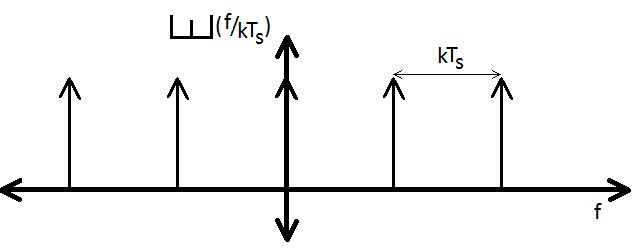
\includegraphics[width=0.5\linewidth]{Pictures/Chapter_2_Lesson_1/Sampling5.png}

So end up with a pulse train in the spectral domain, however the distnace between pusles is no longer the sampling period, but the sampling frequency.  So what have we accomplished here.  We had a continuous time domain signal and we were interested in the resulting spectrum that we obtain when discretize the signal.  We already know that a discrete signal in time domian correpsonds to a periodic signal in frequency domain.  So, but how does it exaclty look and what are the distances between these periodic repetitions, that is something that we just computed cause this distnace will be exaclty the sampling period. SO meaning that in order to compute the spectrum of our signal d(t) what we would need to do is take the fourier transform of our continuous time domain signal x(t) and convoilve it with our impulse response.  Meaning:

\begin{equation*}=\uppercase{\discFunc}(f) = \uppercase{\contFunc}(f)*\Sh(\frac{f}{\samplingFreq}) \end{equation*}

So lets assume X(f) has a certain spectrum something like this:

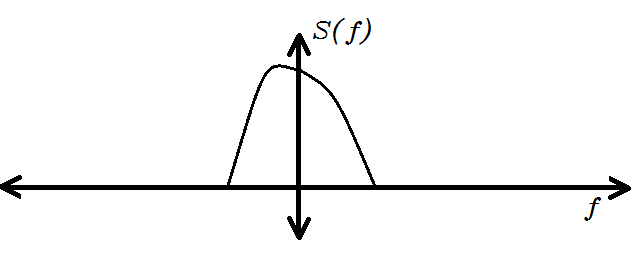
\includegraphics[width=0.5\linewidth]{Pictures/Chapter_2_Lesson_1/Sampling3.png}

and now we convolve this with the fourier transform representaion oif our delta comb

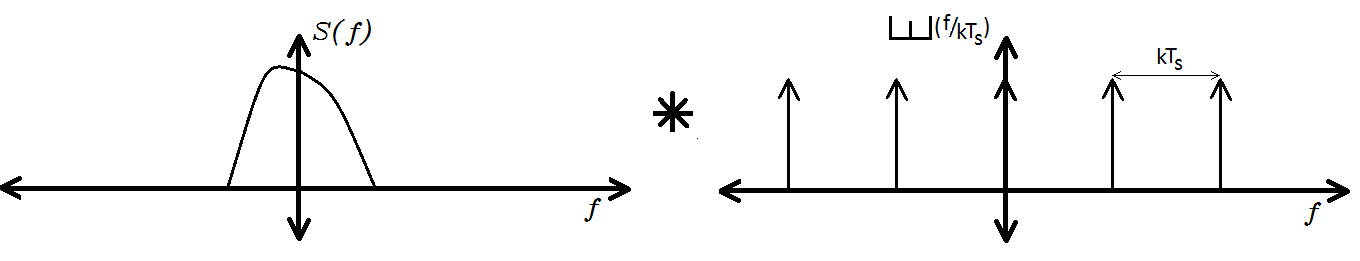
\includegraphics[width=0.5\linewidth]{Pictures/Chapter_2_Lesson_1/Sampling7.png}

SO how would the resulting spectrum look? It would have a periodic representaion.  So what we are drawing here, we can visually derive the sampling theorem.  SO because what happens if we take the sampling frequency too low? If we don not sample our signal often enough.  The replicas of the spectra will overlap meaning that we cannot simply separate the replicas anymore.

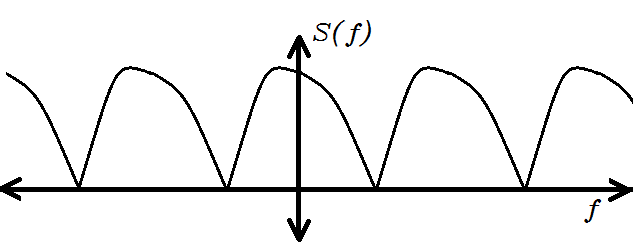
\includegraphics[width=0.5\linewidth]{Pictures/Chapter_2_Lesson_1/Sampling8.png}

SO if fs too low(Ts is too large) then:

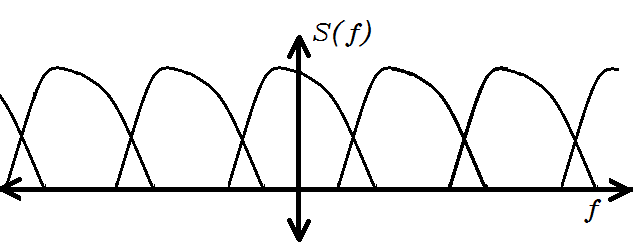
\includegraphics[width=0.5\linewidth]{Pictures/Chapter_2_Lesson_1/Sampling6.png}

 We get our spectrum, except the replicas do not perfectly overlap. This means that we cannot perfectly obtain my signal back again except in trivial examples or specific examples. However, when I have the correctly chosen sampling frequency, then we can simply obtain our signal through lowpass filtering. However this cannot be done when there is an overlap of the signals. SO what does this mean? 
 
 If I choose my smapling frequency, fs, large or equal to 2x's the highest audio frequency, fa. I can perfectly reconstruct the continuous signal x(t) from its discrete representtaion.  
 
 SO this means that if we have a continuous signal, and we sample it with a certain sampling frequency it is true that well you do not sample the samples between two samples. Right so you don not have direct access to these samples, but if the audio bandwidth of this signal is limited it also means that the change between to samples is limited because its a low pass filtered signal in a sense and then if this is the case then you can perfectly interpolate the signal between two samples in a way that you perfectly reconstruct the original continuous signal.
 
 Another way of looking at it or to understand it maybe is that if you have .....what this basically says is that you need a bNDLIMITED SIGNAL that there cannot be a frequency in the signal largeer than fa. that also means that in time domain the change between two samples is limited and so if you fulfill the sampling theorem, you can perfectly reconstruct the signal.
 
 If you obey the Nyquist theorem, tehre is a one to one correspondance between discrete and continuous signals, meaning that we can perfectly reconstruct them.  ANd then if you dont obey it, we get mirror images there will be energy in the signal where it should not be.  If wanted to sample the signal at a lower sample rate, we would need to first apply a low pass.  This would a solution.  Either we could just just a sample frequency high enough, or another thing that we could do if we wanted to choose a lower sample frequency. With speech sounds, we hear these artifacts with high frequency sounds such as s.
 
 SO typical bandwidth that we use.  In telephony, like an ISDN phone but also with your cell phone, we work with sampling rates of about 8khz and then we also low pass filter our signal.  ALthough we have drawn the low pass filter very steep, in practice we cannot realize it this steeply.  So lets say we have speech signals with a bandwidth of up to 16khz.  Then now we use a sampling rate of 8khz, we dont want to havce any information after to 4khz.  But you will not be able to realize low pass filter that has an ideally steep cutoff freequency, but instead, what we would have is something that goes a liitlle more like this... meaning that the spectrum will be distorted up to lower frequencies, and for telephone, the area to where the frequencies are not distorted is 3.4khz. So this is this number here, so theortically speaking, with a sampling frequency of up to 8khz you could recontruct a signal of up to 4khz audio bandwidth, but as you need a vertain lowpass filter that has a certain rolloff the area where the speech is undistorted is only upto 3.4khz.
 
 For music, of course we need higher audio bandwidths,  .....as we said for telephone speech we have 8khz bandwidth, if we have wideband speech telephony, the sampling rate is higher and so the sound quality is better that you can have in a lossless transmission.  Thiese are coding strategies used in some voice over IP clients.  Hifi would be even higher with 44.1kHz, or some standards use 48khz. However at 96khz we are beyond the threshold of hearing and ti makes no sense. 
 
 The next thing that we have to do to discretize a signal, we talked about the discretiaztion on the time axis, but we need to also discrteize the amplitude axis and this.  LATER.
 
 one period no longer fits into one frame  the what happens is, you would basicallc convolve the signal wit ha synch function and you's see samples of the synch function and then you would take discrete samples at theese points.  and then you can imagine that if you have closely spaced sinusoid you will not be able to resiolce those. So a problem is that for the windowed signal, not only do you have one peak at one frequency, you also have what is called spectral leakage so you see energy at frequency components where there is no energy.  and the only way to make this better is to apply tapered anaylsis windows.

For instance a Hamm window or a Hann window because then if you look at the frequency response, you get something that has a certain mainlobe around zero and certain sidebands.  And these sidebands get highly reduced if you tapered analysis window and that basically helps to reduce the spectral leakage effects.  And this is again the same example, the same sinusoid as two slides before and now we see the sinusoid fits the frame length, but still we have a maximum peak where it should be, but you also see that there is energy in the two succesive samples.  SO this is the price that we have t opay for the gain in sideband attenutaion, so you have a wider main lobe meaning that you also have a worsened frequency resolution. SO if you can imagine that if you have a second frequency or a second sinusoid close to it, the frequencies are more likely to mix. But you also see that for a sinusoid that doesnt ideally fit inot the segement, the energy leakage that you would have had a frequencies further away, from the signal frequency would be reduced. 


SO what is the advantage of using such windows? Here you see the time domain window so this is a Hann window this is a Haming window and this is a rectangular window of size 20.  -10 to 10.   so 20ms and here you see its spectral representation where you can see that the higher that this curve is, the more spectral leakage taht we observe and we want to reduce it so we would prefer the red window, the Hann window. However  nothing coes for free. To be able to reduce this spectral leakgae, we also increase the width of the main lobe.  SO here for the rectangular window, its just that steep but the nit does nto reduce that much anymore, but for the other two, for these bell shaped curves, they have a a wider main lobe, but the side band attenutation is increased.  SO somehow we trade off between the spectral resolution awhich is given by the widths of the main lobe and the spectral leakage. SO we can either have a very high spectral resolution with a lot of spectral leakage, or the other way around .  And normally we choose, in a typical situation, the tapered windows.  The rectangualar window is rarely used. 

SPectral Resolution
So the spectral resolution depends on the choice of window, but it also depends on the length of the window.  SO this here, that is the normalized angular frequency its 2pi/N where N is the number of sampüles.  So the length of the window. THe longer the window is so lets say N is very large, then this here the delta phi which is the distacne  between two neighboring bands in frequency becomes much smaller so instead of lets say 200Hz resolution we have 50Hz.  And sometimes you can just take a longer signal if your signal is too short, so we artificailly increase the length of N. How can we do this? Well we take the signal that we have and append a lot of zeros to it.  Thats called zeropadding.  And with that we really increase the number, N so that we increase the number of frequency bins howerver you do not add any addtional infromation, you just add zeros so you do not REALLY increase the spectral resolution but you just increase the sampling. SO here is just ....

so here we have a rectangular window and there are two signals bot consist of two sinusoids with almost the same frequency just a little apart where these two are closer together than these two. YOu can see that for this length, N=16, the DFT is not capable of resolving the two peaks, so what you see when you compute the DFT is 008800008800. You will just see one peak, not two specific ones. While if they are further apart,you can see that these peaks are still resolved.  

so now lets goto zero padding.  So here we have the same signal, but in the lower one, you just increase the number of zeros and what you can see is that the DTFT looks exactly the same, thats the information available in the signal, but its just sampled more often, more frequently so we just sample here, sample there.  So there is no more information, it is just sampled more densely.  Thats the effect of zero padding
% CHAPTER 3 LESSON 3
\clearpage
\section{Discrete Fourier Transform (DFT)}
\label{Discrete Fourier Transform (DFT)}

 The discrete FOurier transform is what we usually work with.  The discrete time FOurier transform that we defined before but the problem here is that if you in  practice you cannot compute it because it is defined as an infinite sum over the signal that you are looking at and in practice you cannot compute an infinite sum, it would take forever literally.  SO what you would have to do is in practice is take a finite time sequence and in a similar way to how we understood sampling again you can think about what does that mean if you chop a certain segment from a signal. And this you can model by multiplying the signal with a rectangular window.
 
 So this would be our time domain signal, with a certain spectrum which can be periodic becasue we have a discrete time fourier transform so this is a discrete signal in time domain giving a continuous and periodic spectrum.  We multiply this with a rectangular window function and this rectangular window function corresponds to a synch function in the frequency domain.  Meaning that if we multiply the two, what you get is a convolutuion of the spectrum with a synch function and this convolution means that you smear your spectrum in the specectral domain,  Meaning that the spectral content will be smeared which also means that your frequency resolution decreases for instance if you have two closely spaced sinuosids and you want to distinguish between them in the frequency domain you need this synch function to be narrow enough so that two signals do not interfere with each other. So lets say 
you have two sinusoidal signals that correspond to two deltas in the spectral domain.  SO we have x1 and x2 which are the sums of two sinusoids. So  now this figure is no longer infintelky log as we would beed it for the discret time FOurier transfom, but we would chop it somewhere.  That means that we will convolve the spectrum with a synch function and then we have a synch function here and a synch function there and you will add the sum of them, meaning that if the synch function gets too broad, then in the resulting spectrum you might get something that looks like this.  Where you are not able to see the two peaks.  This happens if you choose the rectangular window too small.  So in order to increase your spectral resolution you would need more data, in a sense, to find the two sinusoidal components. This is what we learn in this simple example, the trick is that we must know that a multiplecation in the time domain corresponds to convolution in the frequency domain and the fact that a rectangualr function in time domain corresponds to a synch function in the frequency domain .

So now we understand the influence of cutting the spectrum so what do we have here. If we sample the freequency spectrum with sampling period 1/nT then the final time sequence n samples will periodically repeated without and overlap, time domain aliasing. SO what you see here is that the what we are trying to derive here is that the discrete fourier tansform representaion. because in the representaion that we had before, the discret time fourioer  transform,  we had a discrete time representaiton but a continuous frequency representaion now we try to understand what happens if we sample my spectrum, it means that in time domain, my signal will be periodically repeated in the same way that we derived the frequency domain representation and out sampling theorem.

And what this basically means is thta if we discretize oiur spectrum, alos our time domain signal will be repeated and if then also take a rectangular windoww a certain length N, the same way that we did witjh the sampling theorem, we have to take care that when I periodically repeat my spectrum, that these two segments do not overlap. And that correpsonds to how I sample the spectrum in the frequency domain. SO what happens basically, is if you have a discret fourier tansform analysis, that first of allyou look at a windowed part of your time domain signal, then you sample your signal in the frequewncy domain and that corresponds to a periodica represntation of you signal.  If you do use the dft in matlab, then we only look at part of it, the first n sammples both in time domain and in frequency domain, but what you should keep in mind at least in the theory part, that these segemnts will be periodically repeated which is becaue a discrretized signal in time domain correpsonds to a periodic spectrum and a discret frequency domain signal corresponds to a periodic time domain signal. 

And then we have now the discrete fourier transform defintiom where we have bnoth a discrete time domain signal with sample index n and a discrete spectrum with frequency bin index k. And well for the discrete fourier transform, this is what we will mostlay use, for in speech analysis for in this lecture, it'll again have all of these propertioes, Linearity.

In practice, we have fast ways of computing the discrete fourier transform, for instance, the fast fourier transform.  And this is one of the reasons why the discrete fouriertransform is a very often used  spectral representation for speech signals or for audio processing in general  because we have this fast fourier trandform  which is computationally efficient and allows for a fast representaiton of the spectrum of a asignal. And this is one of the basic tools that we use in speech processing. 

Windowing corresponds to the fact that if you chop the signal, it corresponds to the convolution of the function wioth a synch function. For instance, if you have a sinusiod then this would ideally correspond to only one peak in the spectrum, so this  a DFT representaion.  And if the sinusoid fits exactly the window that  youre looking at then also, in the DFT domain, you would see one peak.  Howevre if this is not the case, so again we would have 16 samples inthe time domian, but now the frequency a bit diffeent,